\documentclass{report}
\usepackage[a4paper, portrait, top=20mm, left=20mm, right=20mm, bottom=20mm]{geometry}
\usepackage{graphicx,wrapfig,amsmath,amssymb,algorithm,algpseudocode,caption,subcaption} 

\title{Deep Learning}
\author{Abhijit Amrendra Kumar}
\date{August 2023}

\begin{document}

\maketitle

\chapter{Perceptrons}
\section{Introduction}
\subsection{What is a Perceptron ?}
\noindent Perceptron is a probabilistic model for information storage and organization in the brain.

\begin{figure}[H]
  \centering
  \begin{subfigure}{.5\linewidth}
    \centering
    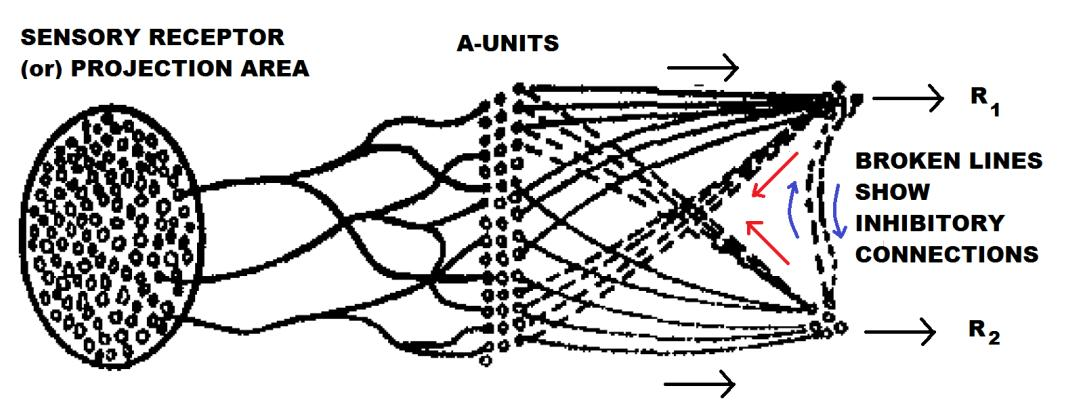
\includegraphics[width=0.8\linewidth]{"images/perc-03.jpg"}
    \label{fig:sub1}
  \end{subfigure}%
  \begin{subfigure}{.5\linewidth}
    \centering
    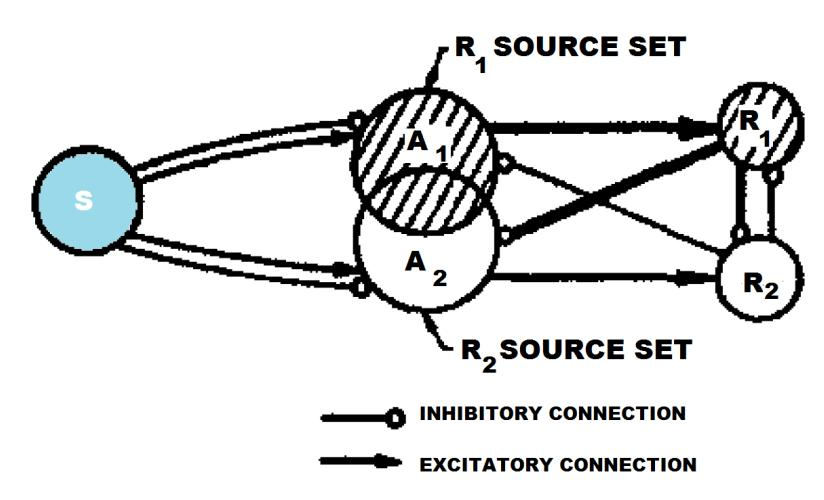
\includegraphics[width=0.5\linewidth]{"images/perc-04.jpg"}
    \label{fig:sub2}
  \end{subfigure}
\end{figure}


\noindent Mathematically, a perceptron is a function that takes input signals and produces an output signal based on the weighted sum of the inputs. These weights are adjusted during learning to enable the perceptron to make accurate classifications or decisions. \\

\noindent The learning rule is inspired by Hebbian learning, a biological learning principle that suggests that synaptic connections between neurons strengthen when those neurons are activated together. In the context of the perceptron, the learning rule updates the weights to minimize the error between the perceptron's output and the desired target output. \\

\noindent Frank Rosenblatt demonstrated that the perceptron can successfully learn linearly separable patterns and achieve convergence within a finite number of iterations. Therefore, the perceptron model can be used for binary classification tasks, where it learns to separate input data points into two classes by finding an optimal decision boundary. Although this model is not used in practice nowadays, it serves as a building block for the modern neural network architectures. \\

\noindent However, Rosenblatt also highlighted the limitations of the perceptron model. He showed that the perceptron is limited to learning linearly separable patterns and cannot handle more complex patterns that require nonlinear decision boundaries. This limitation, known as the \textbf{perceptron convergence theorem}, sparked subsequent research into developing more advanced neural network architectures capable of handling nonlinear problems.

\subsection{Key Assumptions}
\begin{itemize}
  \item Stimuli which are similar will tend to form pathways to same sets of response cells
  \item Stimuli which are dissimilar will tend to form pathways to different sets of response cells
  \item Application of positive and negative reinforcements may facilitate or hinder the formation of connections.
  \item Similarity of stimuli is a dynamically evolving attribute.
\end{itemize}

\section{Perceptron Training}

\subsection{Definitions}
\begin{itemize}
  \item \textbf{Margin of a hyperplane}: The distance between the hyperplane and the data point nearest to it.
  \item \textbf{Margin of a dataset $\gamma$}: The maximum margin possible for that dataset using any weight vector $w$.
\end{itemize}

\subsection{Geometric Intuition}
Given a set of points on a n-dimensional plane, each having one out of two labels $\{+1,-1\}$.

\noindent For visualization, we can use the following figure.
\begin{center}
  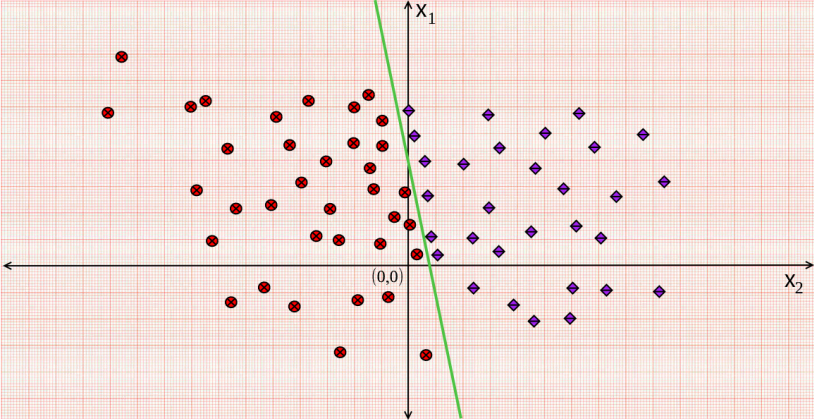
\includegraphics[scale=0.4]{"images/perc-01.png"}
\end{center}

\noindent We want to use the perceptron model to determine a hyperplane that can separate the points based on their labels, i.e. $\{+1,-1\}$.

\subsection{Assumptions}
Based on the above problem, for such a hyperplane to exist, the dataset must satisfy some assumptions.
\begin{itemize}
  \item There must exist atleast 1 hyperplane which separates the points in the dataset based on their labels.
        \begin{itemize}
          \item An example of a 2D dataset which doesn't satisfy the above condition is given below.
                \begin{center}
                  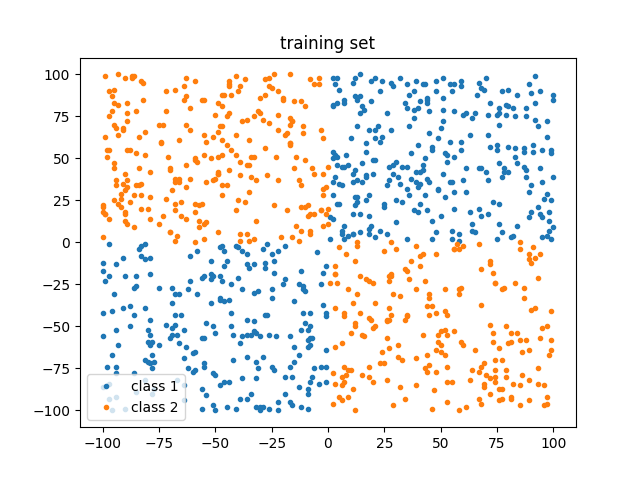
\includegraphics[scale=0.2]{"images/perc-02.png"}
                \end{center}
        \end{itemize}
  \item The margin of the dataset $\gamma > 0$.
        \begin{itemize}
          \item Empirically, $\gamma$ should be large enough for a adequately fast training speed.
        \end{itemize}
\end{itemize}

\subsection{The Model}
Consider the training dataset $D = \{(x^i,y^i)\}_{i=1}^n$.
To solve the above problem, our aim is to train a function/model $h: X \rightarrow Y$. For testing, given $\hat{x}$, the model will be able to predict $\hat{y} = h(\hat{x})$. \\

\noindent Considering the perceptron model, the input is of the form $x = (x_1,x_2,x_3,...x_d) \in \mathbb{R}^d$, the associated weights are of the form $w = (w_1,w_2,w_3,...w_d) \in \mathbb{R}^d$, and the output is of the form $y \in \{+1,-1\}$. \\

\noindent The prediction rule is
$$
  h(x) =
  \begin{cases}
    +1 & \text{if } w^Tx \geq \theta \\
    -1 & \text{if } w^Tx \le \theta  \\
  \end{cases}
$$

\noindent For notational purposes, we can define the following

\begin{align*}
  \Tilde{x} & = (1,x) = (1,x_1,x_2,...x_d) \in \mathbb{R}^{d+1}       \\
  \Tilde{w} & = (1,w) = (-\theta,w_1,w_2,...w_d) \in \mathbb{R}^{d+1}
\end{align*}

\noindent This implies the following modified prediction rule
$$
  H(\Tilde{x}) =
  \begin{cases}
    +1 & \text{if } \Tilde{w}^T\Tilde{x} \geq 0 \\
    -1 & \text{if } \Tilde{w}^T\Tilde{x} \le 0  \\
  \end{cases}
$$

\subsection{The Algorithms}

\begin{algorithm}
  \caption{Algorithm to train a perceptron with a large dataset}
  \begin{algorithmic}
    \State $\tilde{w}^1 \gets 0$ \Comment{Initialize weights}
    \State $\text{for } t \gets 1,2,3,...N \text{ do}$
    \State \hskip1.5em receive $(x^t, y^t), x^t \in \mathbb{R}^d, y^t \in \{+1,-1\}$
    \State \hskip1.5em transform $x^t$ into $\tilde{x}^t = (1,x^t) \in \mathbb{R}^{d+1}$
    \State \hskip1.5em $\hat{y} = \text{perceptron}(\tilde{x}^t,\tilde{w}^t)$ = $sign(\langle \tilde{x}^t,\tilde{w}^t \rangle)$
    \State \hskip1.5em if $\hat{y} \neq y^t$ then
    \State \hskip3em $\tilde{w}^{t+1} = \tilde{w}^t + y^t\tilde{x}^t$
    \State \hskip1.5em else
    \State \hskip3em $\tilde{w}^{t+1} = \tilde{w}^t$
  \end{algorithmic}
\end{algorithm}

\begin{algorithm}
  \caption{Algorithm to train a perceptron with a small dataset}
  \begin{algorithmic}
    \State $\tilde{w}^1 \gets 0$ \Comment{Initialize weights}
    \State $\text{for } t \gets 1,2,3,... \text{ do}$
    \State \hskip1.5em $\text{for } j \gets 1,2,3,...N \text{ do}$
    \State \hskip3em receive $(x^j, y^j), x^j \in \mathbb{R}^d, y^j \in \{+1,-1\}$
    \State \hskip3em transform $x^j$ into $\tilde{x}^j = (1,x^j) \in \mathbb{R}^{d+1}$
    \State \hskip3em $\hat{y} = \text{perceptron}(\tilde{x}^j,\tilde{w}^j)$ = $sign(\langle \tilde{x}^j,\tilde{w}^j \rangle)$
    \State \hskip3em if $\hat{y} \neq y^j$ then
    \State \hskip4.5em $\tilde{w}^{j+1} = \tilde{w}^j + y^j\tilde{x}^j$
    \State \hskip3em else
    \State \hskip4.5em $\tilde{w}^{j+1} = \tilde{w}^j$
  \end{algorithmic}
\end{algorithm}

\subsection{The Procedure}

\noindent Let's try to mathematically formulate the \textbf{linear separability assumption}. \\

\noindent \fbox{\begin{minipage}{\linewidth}
    \noindent \textbf{Linear Separability Assumption}
    \vspace{1mm}
    \hrule
    \vspace{1mm}

    \noindent Let $D = \{(x^t,y^t)\}_{t=1}^{\infty}$ denote the training data where $x^t \in \mathbb{R}^d, y^t \in \{+1,-1\} \ \forall t = 1,2,...$. \\
    \noindent Let $\gamma > 0$ denote the \textbf{margin of the dataset}. Then $\exists \ w^* \in \mathbb{R}^d, w^* \neq 0$, such that
    \begin{align}
       & \langle w^*,x^t \rangle > \gamma, \text{ where } \gamma^t = 1   \\
       & \langle w^*,x^t \rangle < -\gamma, \text{ where } \gamma^t = -1 \\
       & (1.1),(1.2) \implies y^t\langle w^*,x^t \rangle > \gamma
    \end{align}
  \end{minipage}}
\vspace{5mm}

\noindent \textbf{Claim}: If the linear separability assumption holds, the perceptron makes a finite number of mistakes during the run of the algorithm. \\

\noindent \textbf{Proof}: Consider a round $t$ where the perceptron made a mistake. By definition, $w^*$ depends on the dataset, so it is essentially constant in our analysis. The problem lies in figuring out the value of $w^*$. However, let's consider the difference in the dot products $\langle w^*,w^{t+1} \rangle$ and $\langle w^*,w^t \rangle$.

\begin{align}
  \langle w^*,w^{t+1} \rangle - \langle w^*,w^t \rangle & = \langle w^*,w^t + y^tx^t \rangle - \langle w^*,w^t \rangle \\
                                                        & = \langle w^*,y^tx^t \rangle                                 \\
                                                        & = y^t\langle w^*,x^t \rangle                                 \\
\end{align}

\noindent Using the \textbf{linear separability assumption},
\begin{align}
  (1.3) \implies y^t\langle w^*,x^t \rangle                      & > \gamma \\
  \implies \langle w^*,w^{t+1} \rangle - \langle w^*,w^t \rangle & > \gamma
\end{align}

\noindent Now, let's try doing a summation over all the dataset points.
$$
  \overset{N}{\underset{i=1}{\sum}} \langle w^*,w^{t+1} \rangle - \langle w^*,w^t \rangle
$$

\noindent For the rounds having mistakes, $(1.9)$ holds, while for rounds having no mistakes,
$$
  w^{t+1} = w^t \implies \langle w^*,w^{t+1} \rangle - \langle w^*,w^t \rangle = 0
$$

\noindent Let's say the total number of rounds with mistakes is $M$. Hence, our summation changes into
\begin{align}
  \overset{N}{\underset{i=1}{\sum}} \langle w^*,w^{t+1} \rangle - \langle w^*,w^t \rangle          & = \underset{\text{mistakes}}{\sum} \langle w^*,w^{t+1} \rangle - \langle w^*,w^t \rangle \\
  \implies \overset{N}{\underset{i=1}{\sum}} \langle w^*,w^{t+1} \rangle - \langle w^*,w^t \rangle & > M\gamma                                                                                \\
  \implies \langle w^*,w^{N+1} \rangle - \langle w^*,w^1 \rangle                                   & > M\gamma                                                                                \\
  w^1 = 0 \implies \langle w^*,w^{N+1} \rangle                                                     & > M\gamma                                                                                \\
  \implies M\gamma < \langle w^*,w^{N+1} \rangle                                                   & \leq ||w^*||.||w^{N+1}||
\end{align}

\noindent For the rounds having mistakes, let's consider $||w^{t+1}||^2$.
\begin{align}
  ||w^{t+1}||^2 & = ||w^t + y^tx^t||^2                                            \\
                & = (w^t+y^tx^t)^T(w^t+y^tx^t)                                    \\
                & = ||w^t||^2 + ||y^t||^2.||x^t||^2 + 2y^t\langle w^t,x^t \rangle
\end{align}

\noindent We know that the last term is the product of $y^t$ and the prediction value $\hat{y}$. Since this round has the prediction mistake, we can conclude that the last term is \textbf{negative}. Also, we know that $||y^t||^2 = 1$.
\begin{align}
  ||w^{t+1}||^2 - ||w^t||^2 & = ||y^t||^2.||x^t||^2 + 2y^t\langle w^t,x^t \rangle \\
                            & < ||x^t||^2
\end{align}

\noindent Performing a telescopic summation over all rounds with mistakes, and using $w^1 = 0$ yields
\begin{align}
  ||w^{N+1}||^2 < M||x^t||^2
\end{align}

\noindent Realistically, all the points in the dataset can be bounded within a d-dimensional ball, whose radius $R$ is the max L2-norm among all the feature vectors $x^i, i = 1,2,3,...N$.
\begin{align}
  ||w^{N+1}||^2 < M||x^t||^2 & < MR^2 \\
  \implies ||w^{N+1}|| < R\sqrt{M}
\end{align}

\noindent Using $(1.14),(1.22)$, we obtain
\begin{align}
  M\gamma < ||w^*||.||w^{N+1}|| & < R\sqrt{M}||w^*|| \\
  \implies M < ||w^*||^2\cdot R^2/\gamma^2
\end{align}

\noindent To summarize, the following inequality, also known as the \textbf{Perceptron Mistake Bound}, implies an upper bound on the number of mistakes $M$ occuring during the training of a perceptron.
$$
  \boxed{M < ||w^*||^2\cdot R^2/\gamma^2}
$$

\newpage
\subsection{Moving away from Perceptrons | Dealing with the XOR problem}

\begin{itemize}
  \item Multi-layer perceptron
  \item Replacing the $sign(\langle w,x \rangle)$ with other activation functions, like the ReLU function or the sigmoid function.
\end{itemize}

\begin{itemize}
  \item $n_k^l$ denotes the $kth$ neuron at the $lth$ layer.
  \item $w_{i,j}^l$ denotes the weight connecting the neuron in the $(l-1)th$ layer to the $ith$ neuron in the $lth$ layer.
  \item $z_k^l$ denotes the the inner product computed at $n_k^l$.
  \item $a_k^l$ denotes the activation of $n_k^l$.
\end{itemize}

\begin{align}
  z^1 = \begin{bmatrix}
          z_1^1 \\
          z_2^1
        \end{bmatrix} = \begin{bmatrix}
                          w_{11}^1 & w_{12}^1 \\
                          w_{21}^1 & w_{22}^1
                        \end{bmatrix} \begin{bmatrix}
                                        x_1 \\
                                        x_2
                                      \end{bmatrix}
\end{align}

\noindent \textbf{Loss function}: $l: Y\times Y \rightarrow [0,\infty)$

\noindent Some commonly used loss functions are
\begin{align}
  l(y,\hat{y}) := (y-\hat{y})^2 \\
  l(y,\hat{y}) := |y-\hat{y}|   \\
\end{align}

\noindent \textbf{Total loss}: $L = \underset{i=1}{\overset{N}{\sum}}\text{loss}(\hat{y}^i,y^i)$

\noindent We want to minimise the total loss.

\noindent

\end{document}
